\documentclass{standalone} % DO NOT CHANGE THIS
\usepackage{tikz}
\usepackage[utf8]{inputenc}
\usepackage{graphicx}
\usepackage{times}
\usepackage{amssymb}
\usetikzlibrary[arrows.meta, positioning,math, calc, shapes.geometric,intersections, fit, backgrounds, decorations.pathmorphing]

\begin{document}

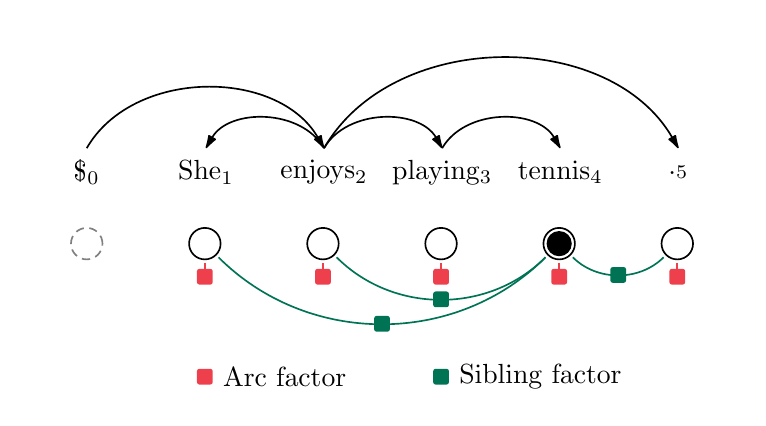
\begin{tikzpicture}[
    word/.style={
            minimum width=1.5cm,
            minimum height=1.5cm,
            inner sep=0pt,
            text width=1.5cm,
            % draw=black
        },
    green connect/.style={
            draw={rgb,255:red,0; green,115; blue,85},
            shorten >= 1pt,
            shorten <= 1pt,
            semithick
        },
    green filled/.style={
            fill={rgb,255:red,0; green,115; blue,85},
        },
    red connect/.style={
            draw={rgb,255:red,238; green,63; blue,77},
            shorten >= 1pt,
            shorten <= 1pt,
            semithick
        },
    red filled/.style={
            fill={rgb,255:red,238; green,63; blue,77},
        },
    dep arrow/.style={
    arrows={-Latex[round,length=6pt,width=3.5pt]},
    semithick
    },
    connect/.style={
            shorten >= -0.5pt,
            shorten <= 1pt,
        },
    ]
    \centering

    \node [word] [anchor=north west, text centered, minimum height=0.6cm] (w0) {\$$_0$};
    \node [word] [anchor=north west, text centered, minimum height=0.6cm] (w1) at ($(w0.north east) + (0.0cm, 0)$) {She$_1$};
    \node [word] [anchor=north west, text centered, minimum height=0.6cm] (w2) at ($(w0.north east) + (1.5cm, 0)$) {enjoys$_2$};
    \node [word] [anchor=north west, text centered, minimum height=0.6cm] (w3) at ($(w0.north east) + (3.0cm, 0)$) {playing$_3$};
    \node [word] [anchor=north west, text centered, minimum height=0.6cm] (w4) at ($(w0.north east) + (4.5cm, 0)$) {tennis$_4$};
    \node [word] [anchor=north west, text centered, minimum height=0.6cm] (w5) at ($(w0.north east) + (6.0cm, 0)$) {.$_5$};

    \node [circle,draw=gray, densely dashed, semithick,inner sep=0pt,minimum size=0.4cm]  (c0) at ($(w0.base) + (0,-0.8cm)$) {};
    \foreach \x in {1,...,5} {
            \node [circle,draw=black,semithick,inner sep=0pt,minimum size=0.4cm]  (c\x) at ($(w0.base) + (1.5cm*\x,-0.8cm)$) {};
            \node [red filled,inner sep=0pt,minimum size=0.2cm,rounded corners=0.3mm]  (f\x) at ($(c\x) - (0,0.42cm)$) {};
            \draw[red connect, thick, connect] (c\x.south) -- (f\x.north);
        }
    \node [circle,draw=none,fill=black, inner sep=0pt, minimum height=0.32cm] at (c4) {};
    \draw[green connect] (c1) to [out=-45, in=-135] node[midway,green filled,inner sep=0pt,minimum size=0.2cm,rounded corners=0.3mm] {} (c4) ;
    \draw[green connect] (c2) to [out=-45, in=-135] node[midway,green filled,inner sep=0pt,minimum size=0.2cm,rounded corners=0.3mm] {} (c4) ;
    \draw[green connect] (c4) to [out=-45, in=-135] node[midway,green filled,inner sep=0pt,minimum size=0.2cm,rounded corners=0.3mm] {} (c5) ;

    \node [red filled,inner sep=0pt,minimum size=0.2cm,rounded corners=0.3mm] (unary) at ($(c1.north)-(0,1.9cm)$) {};
    \node [anchor=west] (unary-text) at ($(unary.east)$) {Arc factor};
    \node [green filled,inner sep=0pt,minimum size=0.2cm,rounded corners=0.3mm] (binary) at ($(c3.north)-(0cm,1.9cm)$) {};
    \node [anchor=west] (binary-text) at ($(binary.east)$) {Sibling factor};


    \draw [dep arrow] [out=120,in=60] (w2.north) to (w1.north);
    \draw [dep arrow] [out=60,in=120] (w0.north) to (w2.north);
    \draw [dep arrow] [out=60,in=120] (w2.north) to (w3.north);
    \draw [dep arrow] [out=60,in=120] (w3.north) to (w4.north);
    \draw [dep arrow] [out=60,in=120] (w2.north) to (w5.north);
\end{tikzpicture}
\end{document}

